\documentclass[0-thesis.tex]{subfiles}

\begin{document}
\section{Device Life Cycle}
\label{sec:device-lifecycle}
% Summarize earlier chapters in a life cycle view
The five key areas discussed in sections \ref{sec:roles}-\ref{sec:upgrading} are all part
of the life cycle of a device. From the moment a new device is deployed in a network to
the point where it is taken out of action possibly several years later, the life cycle
describes a holistic view of the state and operations of devices.

Figure~\ref{fig:lifecycle} summarizes the life cycle of a device from an update
perspective. The figure shows the different stages of a device from being manufactured to
ending its service. There are also annotations showing what needs to be done in each
stage. These stages are discussed in further detail in this section.

\begin{figure}
    \caption{The life cycle of a device.}
    \label{fig:lifecycle}
    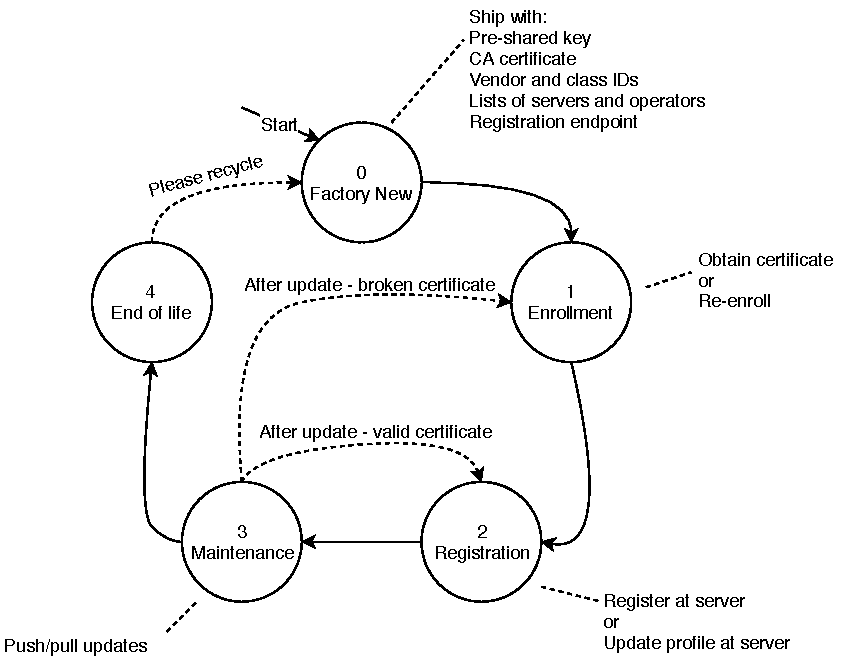
\includegraphics{images/lifecycle.pdf}
\end{figure}

\subsection{Enrollment and Registering}
\label{ssec:enrollment-registering}

A factory new device that is to be installed in an IoT network needs some information in
order to enroll and register at a server. A pre-shared key, CA certificate, vendor and
class IDs, list of servers and operators, and and endpoint for registration is needed.
These parts make sure the device can take part of the network and move to the next step of
the life cycle. 

Entering the enrollment stage, devices obtain certificates by enrolling at the CA. For
this the pre-shared key and CA certificate is needed. After obtaining a certificate the
device can be trusted by the servers and operators, as well as other devices. 

The next stage is registering. The device registers at its designated servers who all
create a profile for the device. The servers can now reach the device, and the device is
ready to be updated, and thus proceeds to the maintenance stage.

\subsection{Maintenance}
\label{ssec:maintenance}
The maintenance state can be expected to last for several years, and this is where the
device receives and applies updates. After an update, a device will either move back to
the enrollment or registration stage. If the certificate is broken after updating, as
discussed in Section~\ref{sec:key-management}, the device move back to the enrollment
stage to obtain a new certificate. After obtaining a new, valid certificate it can update
its profile. If the certificate is still valid after the update, there is no need to
re-enroll and the device moves back to the registration stage, updates the profile at the
servers. Finally the device moves to maintenance once again, and so forth. The device will
remain in the maintenance stage until it either breaks or is taken out of service. If you
are a manufacturer of IoT devices please consider recycling or (securely) re-using
devices, starting the life cycle anew.
\end{document}